\documentclass[a4paper,twoside,10pt,landscape]{article}
\usepackage{multicol}
\usepackage{calc}
\usepackage{ifthen}
\usepackage[landscape]{geometry}
\usepackage{hyperref}
\usepackage{graphicx} % standard LaTeX graphics tool when including figure files
\graphicspath{{images/}}
\usepackage{caption}
\usepackage{multirow}

% To make this come out properly in landscape mode, do one of the following
% 1.
%  pdflatex latexsheet.tex
%
% 2.
%  latex latexsheet.tex
%  dvips -P pdf  -t landscape latexsheet.dvi
%  ps2pdf latexsheet.ps


% If you're reading this, be prepared for confusion.  Making this was
% a learning experience for me, and it shows.  Much of the placement
% was hacked in; if you make it better, let me know...


% 2008-04
% Changed page margin code to use the geometry package. Also added code for
% conditional page margins, depending on paper size. Thanks to Uwe Ziegenhagen
% for the suggestions.

% 2006-08
% Made changes based on suggestions from Gene Cooperman. <gene at ccs.neu.edu>


% To Do:
% \listoffigures \listoftables
% \setcounter{secnumdepth}{0}


% This sets page margins to .5 inch if using letter paper, and to 1cm
% if using A4 paper. (This probably isn't strictly necessary.)
% If using another size paper, use default 1cm margins.
\ifthenelse{\lengthtest { \paperwidth = 11in}}
	{ \geometry{top=.5in,left=.5in,right=.5in,bottom=.5in} }
	{\ifthenelse{ \lengthtest{ \paperwidth = 297mm}}
		{\geometry{top=1cm,left=1cm,right=1cm,bottom=1cm} }
		{\geometry{top=1cm,left=1cm,right=1cm,bottom=1cm} }
	}

% Turn off header and footer
\pagestyle{empty}
 

% Redefine section commands to use less space
\makeatletter
\renewcommand{\section}{\@startsection{section}{1}{0mm}%
                                {-1ex plus -.5ex minus -.2ex}%
                                {0.5ex plus .2ex}%x
                                {\normalfont\large\bfseries}}
\renewcommand{\subsection}{\@startsection{subsection}{2}{0mm}%
                                {-1explus -.5ex minus -.2ex}%
                                {0.5ex plus .2ex}%
                                {\normalfont\normalsize\bfseries}}
\renewcommand{\subsubsection}{\@startsection{subsubsection}{3}{0mm}%
                                {-1ex plus -.5ex minus -.2ex}%
                                {1ex plus .2ex}%
                                {\normalfont\small\bfseries}}
\makeatother

% Define BibTeX command
\def\BibTeX{{\rm B\kern-.05em{\sc i\kern-.025em b}\kern-.08em
    T\kern-.1667em\lower.7ex\hbox{E}\kern-.125emX}}

% Don't print section numbers
%\setcounter{secnumdepth}{0}


\setlength{\parindent}{0pt}
\setlength{\parskip}{0pt plus 0.5ex}


% -----------------------------------------------------------------------

\begin{document}

\raggedright
\footnotesize
\begin{multicols}{3}


% multicol parameters
% These lengths are set only within the two main columns
%\setlength{\columnseprule}{0.25pt}
\setlength{\premulticols}{1pt}
\setlength{\postmulticols}{1pt}
\setlength{\multicolsep}{1pt}
\setlength{\columnsep}{2pt}

\begin{center}
     \Large{\textbf{Scala Cheat Sheet}} \\
\end{center}


\section{Scala Class Hierarchy}
\begin{center}
    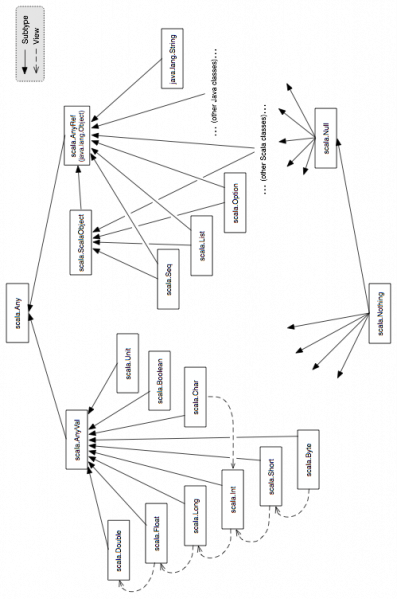
\includegraphics[scale=.80]{classhierarchy.png}
    \captionof{figure}{Scala class hierarchy, source: \url{http://docs.scala-lang.org/tutorials/tour/unified-types.html}}
    \label{fig:scala-class-hierarchy}
\end{center}


\section{Scala Collections}


\subsection{Scala Collections Hierarchy}

\begin{center}
    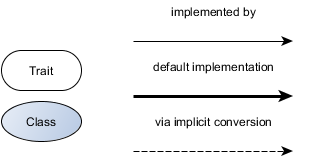
\includegraphics[scale=.40]{legend.png}
\end{center}

\begin{center}
    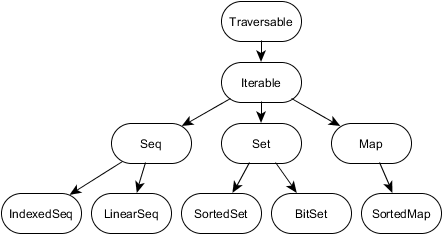
\includegraphics[scale=.50]{scala-collection.png}
    \captionof{figure}{scala.collection}
    \label{fig:scala-collection}
\end{center}

\begin{center}
    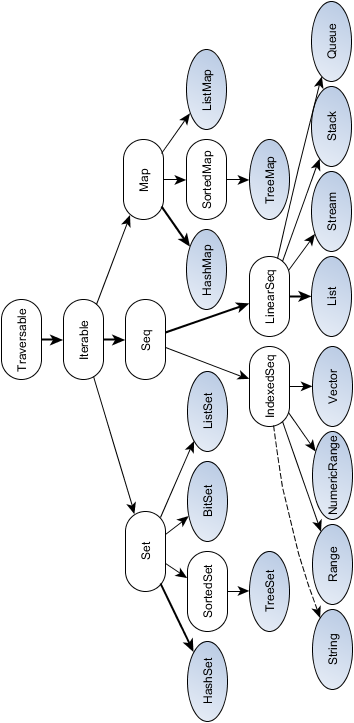
\includegraphics[scale=.65]{scala-collection-immutable.png}
    \captionof{figure}{scala.collection.immutable}
    \label{fig:scala-collection-immutable}
\end{center}

\begin{center}
    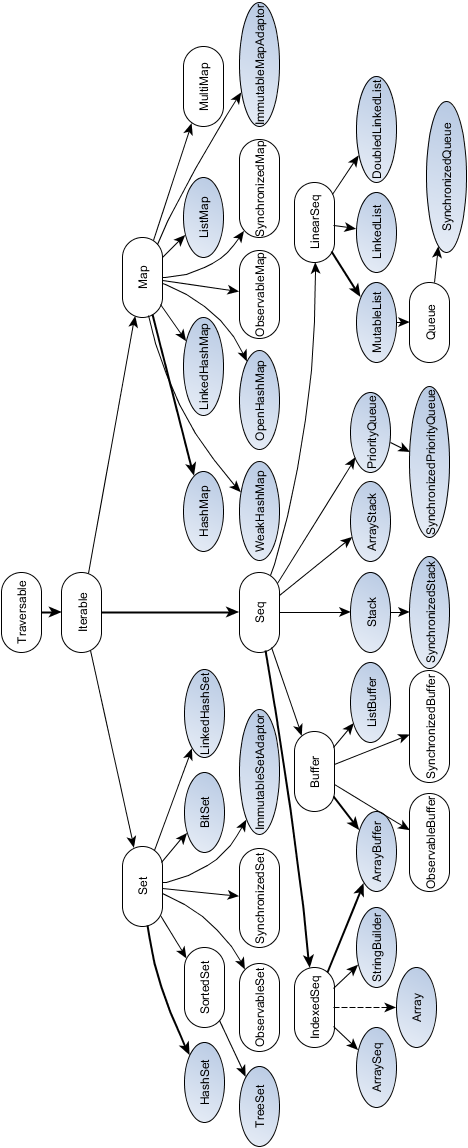
\includegraphics[scale=.60]{scala-collection-mutable.png}
    \captionof{figure}{scala.collection.mutable}
    \label{fig:scala-collection-mutable}
\end{center}


\subsection{Trait \texttt{Traversable}}
\begin{center}
\captionof{table}{Methods in \texttt{Traversable}}
\begin{tabular}{@{}lp{6.5cm}@{}}
\hline\noalign{\smallskip}
\textbf{Category} & \textbf{Methods} \\
\noalign{\smallskip}\hline\noalign{\smallskip}
\textbf{Abstract} & \texttt{xs foreach f}\\
\textbf{Addition} & \texttt{xs ++ ys}\\
\textbf{Maps} & \texttt{xs map f, xs flatMap f, xs collect f}\\
\textbf{Conversions} & \texttt{toArray, toList, toIterable, toSeq, toIndexedSeq, toStream, toSet, toMap}\\
\textbf{Size info} & \texttt{isEmpty, nonEmpty, size, hasDefiniteSize}\\
\textbf{Element} & \texttt{head, headOption, last, lastOption},\\
\textbf{Retrieval} & \texttt{xs find p}\\
\textbf{Sub-} & \texttt{xs.tail, xs.init, xs slice (from, to)},\\
\textbf{collection} & \texttt{xs take n, xs drop n, xs takeWhile p, xs dropWhile p, xs filter p, xs withFilter p, xs filterNot p}\\
\textbf{Subdivision} & \texttt{xs splitAt n, xs span p, xs partition p, xs groupBy f}\\
\textbf{Element} & \texttt{xs forall p, xs exists p, xs count p}\\
\textbf{Condition} & \\
\textbf{Fold} & \texttt{(z /: xs)(op), (xs :\ z)(op), xs.foldLeft(z)(op), xs.foldRight(z)(op), xs reduceLeft op, xs reduceRight op}\\
\textbf{Specific Fold} & \texttt{xs.sum, xs.product, xs.min, xs.max}\\
\textbf{String} & \texttt{xs addString (b, start, sep, end), xs mkString (start, sep, end), xs.stringPrefix}\\
\textbf{View} & \texttt{xs.view, xs view (from, to)}\\
\noalign{\smallskip}\hline
\end{tabular}
Reference: \url{http://docs.scala-lang.org/overviews/collections/trait-traversable.html}
\end{center}


\subsection{Trait \texttt{Iterable}}
All methods in this trait are defined in terms of an an abstract method, \texttt{iterator}, which yields the collection’s elements one by one.

\begin{center}
\captionof{table}{Methods in \texttt{Iterable}}
\begin{tabular}{@{}lp{6cm}@{}}
\hline\noalign{\smallskip}
\textbf{Category} & \textbf{Methods} \\
\noalign{\smallskip}\hline\noalign{\smallskip}
\textbf{Abstract} & \texttt{xs.iterator}\\
\textbf{Iterator} & \texttt{xs grouped n, xs sliding n}\\
\textbf{Subcollection} & \texttt{xs takeRight n, xs dropRight n}\\
\textbf{Zipper} & \texttt{xs zip ys, xs zipAll (ys, x, y), xs.zipWithIndex}\\
\textbf{Comparison} & \texttt{xs sameElements ys}\\
\noalign{\smallskip}\hline
\end{tabular}
Reference: \url{http://docs.scala-lang.org/overviews/collections/trait-iterable.html}
\end{center}

In the inheritance hierarchy below \texttt{Iterable} you find three traits: \texttt{Seq}, \texttt{Set}, and \texttt{Map}. A common aspect of these three traits is that they all implement the \texttt{PartialFunction} trait with its \texttt{apply} and \texttt{isDefinedAt} methods. However, the way each trait implements \texttt{PartialFunction} differs.


\subsection{Seq}
All methods in this trait are defined in terms of an an abstract method, \texttt{iterator}, which yields the collection’s elements one by one.

\begin{center}
\captionof{table}{Methods in \texttt{Seq}}
\begin{tabular}{@{}lp{6.5cm}@{}}
\hline\noalign{\smallskip}
\textbf{Category} & \textbf{Methods} \\
\noalign{\smallskip}\hline\noalign{\smallskip}
\textbf{Indexing and} & \texttt{xs(i), xs isDefinedAt i, xs.length,}\\
\textbf{Length} & \texttt{xs.lengthCompare ys, xs.indices}\\
\textbf{Index Search} & \texttt{xs indexOf x, xs lastIndexOf x, xs indexOfSlice ys, xs lastIndexOfSlice ys, xs indexWhere p, xs segmentLength (p, i), xs prefixLength p}\\
\textbf{Addition} & \texttt{x +: xs, xs :+ x, xs padTo (len, x)}\\
\textbf{Update} & \texttt{xs patch (i, ys, r), xs updated (i, x), xs(i) = x}(only available for \texttt{mutable.Seq}s)\\
\textbf{Sorting} & \texttt{xs.sorted, xs sortWith lt, xs sortBy f}\\
\textbf{Reversal} & \texttt{xs.reverse, xs.reverseIterator, xs reverseMap f}\\
\textbf{Comparison} & \texttt{xs startsWith ys, xs endsWith ys, xs contains x, xs containsSlice ys, (xs corresponds ys)(p)}\\
\textbf{Multiset} & \texttt{xs intersect ys, xs union ys, xs diff ys, xs.distinct}\\
\noalign{\smallskip}\hline
\end{tabular}
Reference: \url{http://docs.scala-lang.org/overviews/collections/seqs.html}
\end{center}

Trait \texttt{Seq} has two subtraits \texttt{LinearSeq}, and \texttt{IndexedSeq}. These do not add any new operations, but each offers different performance characteristics: A linear sequence has efficient \texttt{head} and \texttt{tail} operations, whereas an indexed sequence has efficient \texttt{apply}, \texttt{length}, and (if mutable) \texttt{update} operations. Frequently used linear sequences are \texttt{immutable.List} and \texttt{immutable.Stream}. Frequently used indexed sequences are \texttt{scala.Array} and \texttt{mutable.ArrayBuffer}. The \texttt{Vector} class provides an interesting compromise between indexed and linear access. It has both effectively constant time indexing overhead and constant time linear access overhead. Because of this, vectors are a good foundation for mixed access patterns where both indexed and linear accesses are used. 

\begin{center}
\captionof{table}{Methods in \texttt{Buffer}}
\begin{tabular}{@{}lp{6.5cm}@{}}
\hline\noalign{\smallskip}
\textbf{Category} & \textbf{Methods} \\
\noalign{\smallskip}\hline\noalign{\smallskip}
\textbf{Addition} & \texttt{buf += x, buf += (x, y, z), buf ++= xs, x +=: buf, xs ++=: buf, buf insert (i, x), buf insertAll (i, xs)}\\
\textbf{Removal} & \texttt{buf -= x, buf remove i, buf remove (i, n), buf trimStart n, buf trimEnd n, buf.clear()}\\
\textbf{Cloning} & \texttt{buf.clone}\\
\noalign{\smallskip}\hline
\end{tabular}
\end{center}


\subsection{Set}
\begin{center}
\captionof{table}{Methods in \texttt{Set}}
\begin{tabular}{@{}lp{6.5cm}@{}}
\hline\noalign{\smallskip}
\textbf{Category} & \textbf{Methods} \\
\noalign{\smallskip}\hline\noalign{\smallskip}
\textbf{Test} & \texttt{xs contains x, xs(x), xs subsetOf ys}\\
\textbf{Addition} & \texttt{xs + x, xs + (x, y, z), xs ++ ys}\\
\textbf{Removal} & \texttt{xs - x, xs - (x, y, z), xs -- ys, xs.empty}\\
\textbf{Set operation} & \texttt{xs \& ys, xs intersect ys, xs | ys, xs union ys, xs \&~ ys, xs diff ys}\\
\noalign{\smallskip}\hline
\end{tabular}
Reference: \url{http://docs.scala-lang.org/overviews/collections/sets.html}
\end{center}

Mutable sets offer in addition methods to add, remove, or update elements, which are summarized in below.

\begin{center}
\captionof{table}{Methods in \texttt{mutable.Set}}
\begin{tabular}{@{}lp{6.5cm}@{}}
\hline\noalign{\smallskip}
\textbf{Category} & \textbf{Methods} \\
\noalign{\smallskip}\hline\noalign{\smallskip}
\textbf{Addition} & \texttt{xs += x, xs += (x, y, z), xs ++= ys, xs add x}\\
\textbf{Removal} & \texttt{xs -= x, xs -= (x, y, z), xs --= ys, xs remove x, xs retain p, xs.clear()}\\
\textbf{Update} & \texttt{xs(x) = b}\\
\textbf{Cloning} & \texttt{xs.clone}\\
\noalign{\smallskip}\hline
\end{tabular}
\end{center}


\subsection{Map}
\begin{center}
\captionof{table}{Methods in \texttt{Map}}
\begin{tabular}{@{}lp{6cm}@{}}
\hline\noalign{\smallskip}
\textbf{Category} & \textbf{Methods} \\
\noalign{\smallskip}\hline\noalign{\smallskip}
\textbf{Lookup} & \texttt{ms get k, ms(k), ms getOrElse (k, d), ms contains k, ms isDefinedAt k}\\
\textbf{Addition} & \texttt{ms + (k -> v), ms + (k -> v, l -> w), ms ++ kvs}\\
\textbf{Removal} & \texttt{ms - k, ms - (k, 1, m), ms -- ks}\\
\textbf{Update} & \texttt{ms updated (k, v)}\\
\textbf{Subcollection} & \texttt{ms.keys, ms.keySet, ms.keyIterator, ms.values, ms.valuesIterator}\\
\textbf{Transformation} & \texttt{ms filterKeys p, ms mapValues f}\\
\noalign{\smallskip}\hline
\end{tabular}
Reference: \url{http://docs.scala-lang.org/overviews/collections/maps.html}
\end{center}

\begin{center}
\captionof{table}{Methods in \texttt{mutable.Map}}
\begin{tabular}{@{}lp{6cm}@{}}
\hline\noalign{\smallskip}
\textbf{Category} & \textbf{Methods} \\
\noalign{\smallskip}\hline\noalign{\smallskip}
\textbf{Addition} & \texttt{ms += (k -> v), ms += (k -> v, l -> w), ms ++= kvs, }\\
\textbf{Removal} & \texttt{ms -= k, ms -= (k, l, m), ms --= ks, ms remove k, ms retain p, ms.clear()}\\
\textbf{Update} & \texttt{ms(k) = v, ms put (k, v), ms getOrElseUpdate (k, d)}\\
\textbf{Transformation} & \texttt{ms transform f}\\
\textbf{Cloning} & \texttt{xs.clone}\\
\noalign{\smallskip}\hline
\end{tabular}
\end{center}


\rule{0.3\linewidth}{0.25pt}
\scriptsize

Copyright \copyright\ 2014 soulmachine

Github: \url{https://github.com/soulmachine/scala-cheat-sheet} 

My blog: \url{http://www.soulmachine.me}

Last update: \today


\end{multicols}
\end{document}
